\subsection{Conceptos básicos}
\label{c:fundamentos_musicales}

%----------------------------------------------------------------------------
% NOTACIÓN MUSICAL
%----------------------------------------------------------------------------
\subsubsection{Notación musical}
La \textbf{\gls{notación musical}}~\cite{wikipedia_notacion_musical} es el sistema de escritura que se utiliza con el fin de representar las notas musicales que conforman una canción. Estas pueden ser gráficas o alfabeticas, siendo las mas populares la \textbf{notación en pentagrama} \figref{fig:pentagrama}, la \textbf{\gls{notación latina}} y la \textbf{\gls{notación anglosajona}} \tabref{tab:equivalencia_notacion_ang_lat}.

\begin{figure}[H]
    \scriptsize
    %\centering
    % --- Figura a la izquierda ---
    \begin{minipage}[t]{0.48\textwidth}
        \vspace{0pt} % fuerza la alineación superior
        \centering
        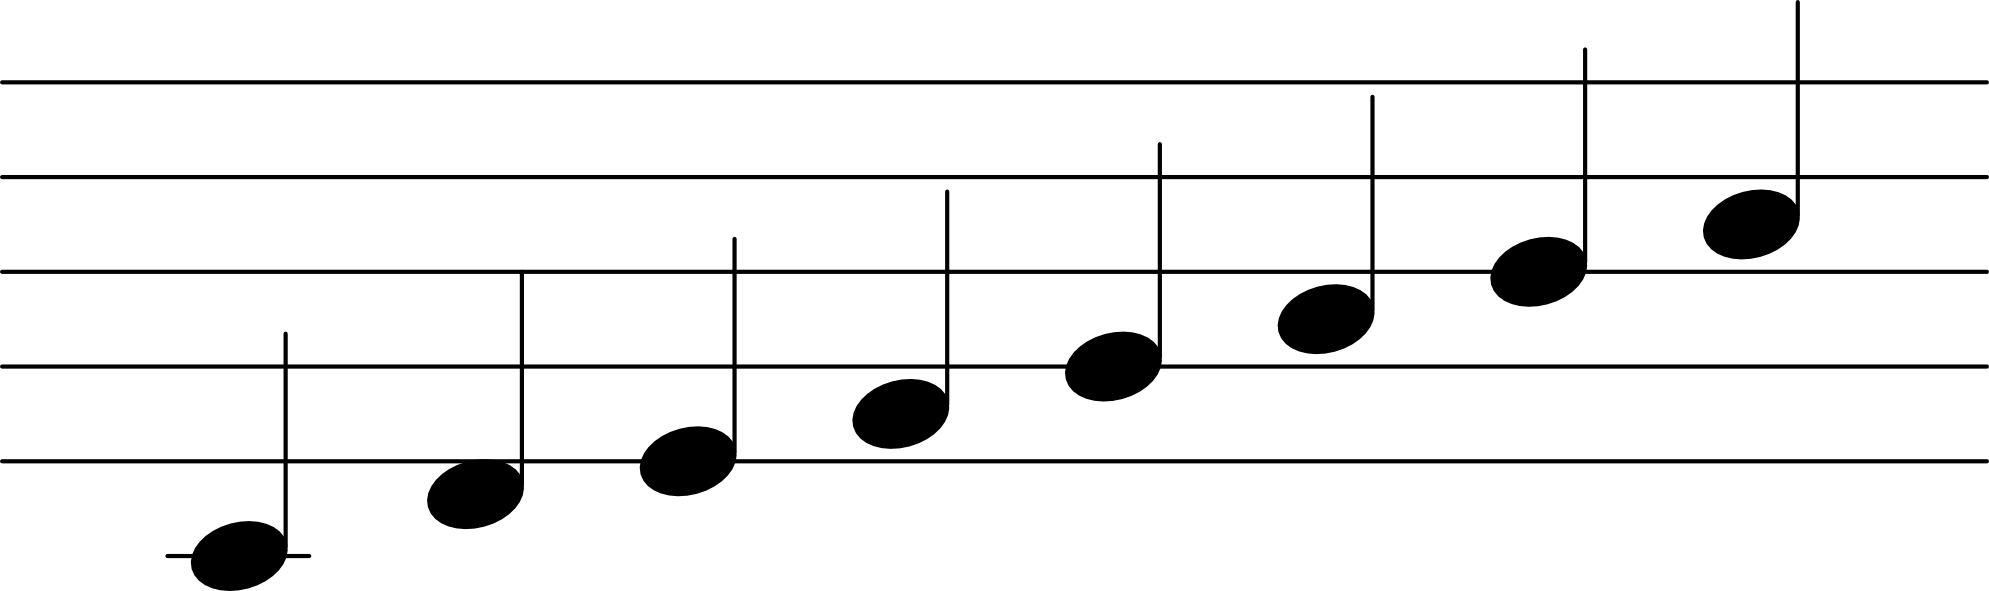
\includegraphics[width=\textwidth]{Ilustraciones/estado/pentagrama.jpg}
        \caption{Notación en pentagrama}\label{fig:pentagrama}
    \end{minipage}
    \hfill
    % --- Tabla a la derecha ---
    \begin{minipage}[t]{0.48\textwidth}
        % fuerza la alineación superior
        \vspace{23pt} 
        \centering
        \begin{tabular}{l c c c c c c c}
            \hline
            \textbf{Notación} & \multicolumn{7}{c}{\textbf{Notas}} \\
            \hline
            Latina & $Do$ & $Re$ & $Mi$ & $Fa$ & $Sol$ & $La$ & $Si$ \\
            Anglosajona & $C$ & $D$ & $E$ & $F$ & $G$ & $A$ & $B$ \\
            \hline
        \end{tabular}
        \captionof{table}{Notación latina y anglosajona}\label{tab:equivalencia_notacion_ang_lat}
    \end{minipage}
\end{figure}

\subsubsection{Notas musicales}
En teoría musical se identifican 7 notas naturales \textit{(e.g. teclas blancas del piano)}, entre las cuales se encuentran 5 notas llamadas \textbf{alteraciones} \textit{(e.g. teclas negras del piano)}. Distinguimos dos tipos de:

\begin{itemize}
    \item \textbf{Sostenido}, representado generalmente con el simbolo $\sharp$, se refiere a la nota contigua aguda \emph{(e.g. en el piano Do$\sharp$ es la tecla negra a la derecha de Do)}.
    
    \item \textbf{Bemol}, representado generalmente con el simbolo $\flat$, se refiere la la nota contigua grave \emph{(e.g. en el piano Re$\flat$ es la tecla negra a la izquierda de Re)}.
\end{itemize}

De este modo, podemos afirmar la existencia de 12 notas \figref{fig:piano_notas}.

\begin{figure}[H]
    \centering
    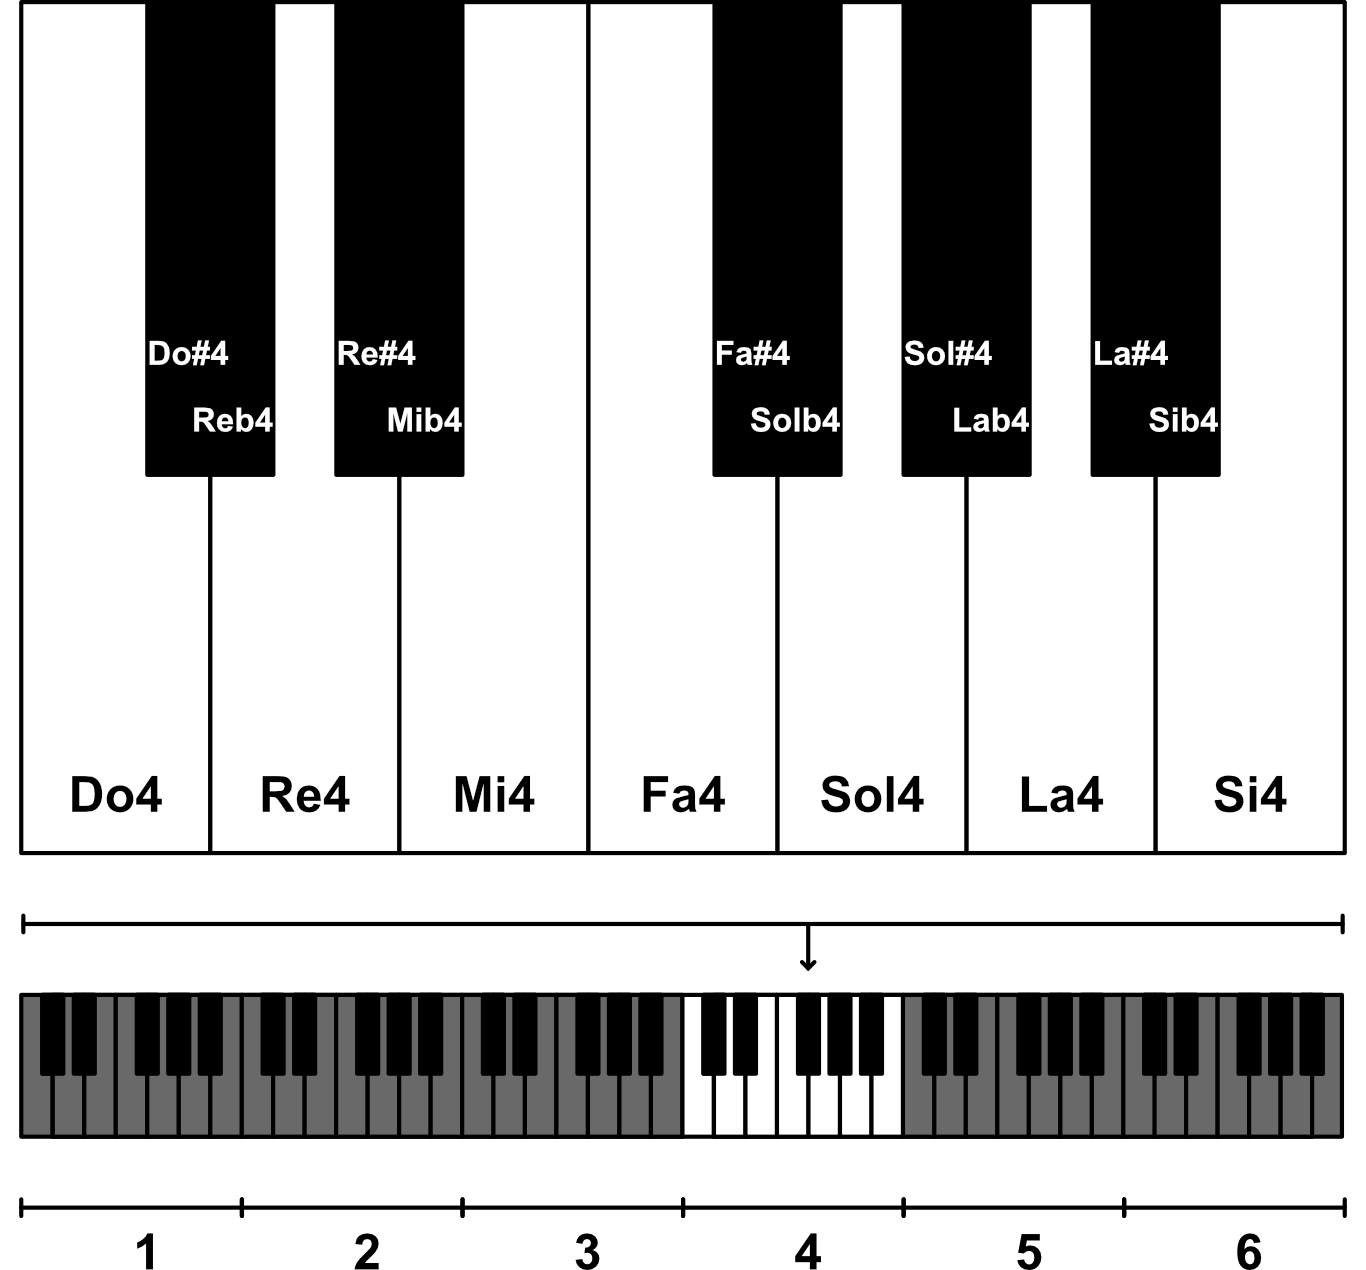
\includegraphics[width=0.5\textwidth]{Ilustraciones/estado/piano_cromatica.jpg}
    \caption{Notas en un piano}\label{fig:piano_notas}
\end{figure}

La distribución de las alteraciones no es arbitraria y debemos introducir el concepto de distancia entre notas:

\begin{itemize}
    \item El \textbf{\gls{semitono}}, que es la distancia mínima entre dos notas contiguas \emph{(e.g. la distancia entre dos teclas adyacentes del piano)}.

    \item El \textbf{\gls{tono}}, equivalente a dos semitonos \emph{(e.g. la distancia entre dos teclas blancas que tienen una tecla negra entre ellas)}.
\end{itemize}

Una alteración se ubicará entre dos notas naturales con una distancia de 1 tono \textit{(i.e. dos semitonos)} \tabref{tab:notas}.

\begin{table}[H]
        \centering
        \scriptsize
        \caption{Notas naturales, alteraciones y semitonos}\label{tab:notas}
        \begin{tabular}{l c c c c c c c c c c c c c}
        \hline
        \textbf{Naturales} & $Do$ & & $Re$ & & $Mi$ & $Fa$ & & $Sol$ & & $La$ & & $Si$ \\
        \textbf{Alteraciones} & & $Do\sharp$ & & $Re\sharp$ & & & $Fa\sharp$ & & $Sol\sharp$ & & $La\sharp$ & \\
        \textbf{Semitono} & 0 & 1 & 2 & 3 & 4 & 5 & 6 & 7 & 8 & 9 & 10 & 11 \\
        
        \hline
    \end{tabular}
\end{table}

%----------------------------------------------------------------------------
% ESCALA MUSICAL
%----------------------------------------------------------------------------
\subsubsection{Escala musical}
Dado un conjunto de notas, su orden en una secuencia se conoce como \textbf{\gls{escala musical}}~\cite{wikipedia_escala_musical}, caracterizada por:

\begin{itemize}
    \item Poseer un orden en sentido ascendente (de grave a agudo) o descendente (de agudo a grave).
    \item Definir una nota inicial o \textbf{tónica}.
    \item Seguir un patrón de distancias.
\end{itemize}

Además, podemos distinguir el concepto de \textbf{octava} que es el intervalo de notas entre dos iguales \emph{e.g. de Do a Do'}. Este invervalo puede variar según la escala:

\begin{itemize}
    \item La \textbf{escala diatónica}, conformada por 7 notas siguiendo el patrón: tono, tono, semitono, tono, tono, tono y semitono. Cada nota posee un \textbf{grado} que actúa como índice y indicador de la distancia a la tónica. Cada grado posee también un nombre propio \tabref{tab:escala_diatonica}.

    \begin{table}[H]
        \centering
        \scriptsize
        \caption{Escalas diatónicas y octavas con tónicas en $Do$ y en $Re$}\label{tab:escala_diatonica}
        \begin{tabular}{l c c c c c c c c}
            \hline
            & \textbf{I} & \textbf{II} & \textbf{III} & \textbf{IV} & \textbf{V} & \textbf{VI} & \textbf{VII} & \textbf{VIII} \\
            & {\tiny Tónica} & {\tiny Supertónica} & {\tiny Mediante} & {\tiny Subdominante} & {\tiny Dominante} & {\tiny Supermediante} & {\tiny Sensible} & {\tiny Octava}  \\
            \hline
            Escala & $Do$ & $Re$ & $Mi$ & $Fa$ & $Sol$ & $La$ & $Si$ &  \\
            Octava & $Do$ & $Re$ & $Mi$ & $Fa$ & $Sol$ & $La$ & $Si$ & $Do'$  \\
            \hline
            Escala & $Re$ & $Mi$ & $Fa\sharp$ & $Sol$ & $La$ & $Si$ & $Do$ &  \\
            Octava & $Re$ & $Mi$ & $Fa\sharp$ & $Sol$ & $La$ & $Si$ & $Do$ & $Re'$  \\
            \hline
        \end{tabular}
    \end{table}
    
    \item La \textbf{escala cromática}, conformada por 12 notas siguiendo un patrón de 12 semitonos \tabref{tab:escala_cromatica}
    
    \begin{table}[H]
        \centering
        \caption{Escalas cromáticas y octavas con tónicas en $Do$ y en $Re$}\label{tab:escala_cromatica}
        \scriptsize
        \begin{tabular}{l c c c c c c c c c c c c c}
            \hline
            Escala & $Do$ & $Do\sharp$ & $Re$ & $Re\sharp$ & $Mi$ & $Fa$ & $Fa\sharp$ & $Sol$ & $Sol\sharp$ & $La$ & $La\sharp$ & $Si$ \\
            Octava & $Do$ & $Do\sharp$ & $Re$ & $Re\sharp$ & $Mi$ & $Fa$ &
            $Fa\sharp$ & $Sol$ & $Sol\sharp$ & $La$ & $La\sharp$ & $Si$ & $Do'$ \\
            \hline
            Escala & $Re$ & $Re\sharp$ & $Mi$ & $Fa$ & $Fa\sharp$ & $Sol$ & $Sol\sharp$ & $La$ & $La\sharp$ & $Si$ & $Do$ & $Do\sharp$ \\
            Octava & $Re$ & $Re\sharp$ & $Mi$ & $Fa$ & $Fa\sharp$ & $Sol$ & $Sol\sharp$ & $La$ & $La\sharp$ & $Si$ & $Do$ & $Do\sharp$ & $Re'$ \\
            \hline
        \end{tabular}
    \end{table}
\end{itemize}

%----------------------------------------------------------------------------
% ACORDES
%----------------------------------------------------------------------------
\subsubsection{Acordes}
Un \textbf{\gls{acorde}}~\cite{wikipedia_acorde} es un conjunto de tres o más notas diferentes que conforman una unidad armónica. Entre los más populares encontramos las \textbf{tríadas} y \textbf{cuatríadas} (o \textbf{séptima}), construídos con tres y cuatro notas respectivamente. 

Para construir un acorde debemos seleccionar una \textbf{\gls{cualidad}} que indicará las distancias en semitonos de las notas \tabref{tab:acordes_cualidades}.

\begin{table}[H]
    \centering
    \caption{Modalidades de acordes}\label{tab:acordes_cualidades}
    \scriptsize
    \begin{tabular}{l c l}
        \hline
        \textbf{Cualidad} & \textbf{Símbolo} & \textbf{Semitonos} \\
        \hline
        Mayor & M & 0, 4, 7 \\
        Menor & m & 0, 3, 7 \\
        Aumentado & aug & 0, 4, 8 \\
        Disminuido & dim & 0, 3, 6 \\
        Séptima & 7 & 0, 4, 7, 10 \\
        Séptima mayor & M7 & 0, 4, 7, 11 \\
        Menor séptima & m7 & 0, 3, 7, 10 \\
        Menor séptima mayor & mM7 & 0, 3, 7, 11 \\
        \hline
    \end{tabular}
\end{table}

Por tanto, para tocar el acorde de $Do Mayor$ (también conocido como DoM o simplemente $Do$), establecemos como tónica la nota $Do$, y seleccionamos las notas correspondientes a las distancias en semitonos 0, 4, 7: es decir, $Do$, $Mi$ y $Sol$ \figref{fig:piano_acorde_doM}.

\begin{figure}[H]
    \centering
    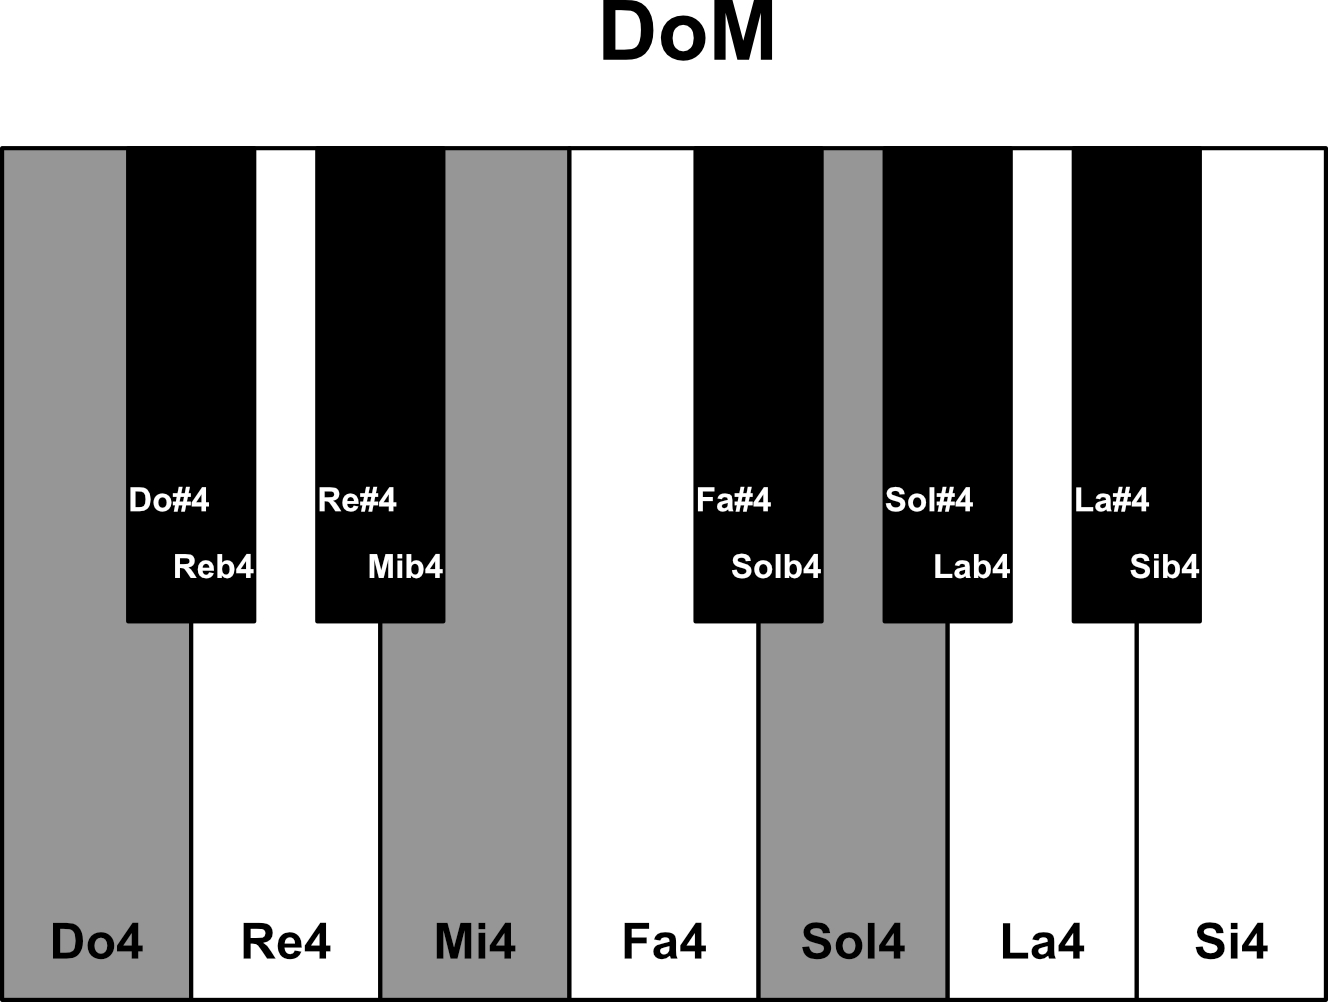
\includegraphics[width=0.5\textwidth]{Ilustraciones/estado/piano_doM.jpg}
    \caption{Acorde de $Do Mayor$ en piano}\label{fig:piano_acorde_doM}
\end{figure}

A una sucesión de acordes lo llamamos \textbf{\gls{progresión}}~\cite{wikipedia_progresion} \emph{(e.g. una progresión popular en el folclore canario es ReM, SolM y LaM)}.

Conocidos los conceptos de acorde y progresión, podemos introducir la \textbf{\gls{transposición}}. Dado un \textbf{acorde raiz}, podemos mover la tónica un semitono a la izquierda o a la derecha para obtener el acorde traspuesto. Si hablamos de una progresión, se realizará la operación anterior en todos los acordes que lo conforman \tabref{tab:transposicion_acordes_progresiones}.

\begin{table}[H]
    \centering
    \caption{Transposición un acorde y una progresión}\label{tab:transposicion_acordes_progresiones}
    \scriptsize
    \begin{tabular}{l l l}
        \hline
        \textbf{Transposición} & \textbf{Acorde} & \textbf{Progresión} \\
        \hline
        Raíz & $DoM$ & $DoM–FaM–SolM$ \\
        +1 & \textit{Do$\sharp$M} & \textit{Do$\sharp$M–Fa$\sharp$M–Sol$\sharp$M} \\
        +2 & \textit{ReM} & \textit{ReM–SolM–LaM} \\
        \hline
    \end{tabular}
\end{table}

%----------------------------------------------------------------------------
% TONALIDAD
%----------------------------------------------------------------------------
\subsubsection{Tonalidad}
La \textbf{tonalidad}~\cite{wikipedia_tonalidad} es un conjunto de notas que, relaciona una escala diatónica con acordes. De este modo podemos realizar asociaciones como:

\begin{itemize}
    \item \textbf{¿A qué tonalidad pertenece un acorde?} 
      El acorde de \textit{Re menor}, construido con las notas $Re$, $Mi$ y $Sol$, 
      pertenece a la tonalidad de \textit{DoM}, ya que todas sus notas forman parte de dicha tonalidad.
    \item \textbf{¿Que acordes pertenecen a una tonalidad?}
      Para la tonalidad de \textit{Do Mayor}, perteneceran solo los acordes cuyas notas se encuentre en su escala, como \textit{DoM}, \textit{Rem}\dots
\end{itemize}

Además, la tonalidad nos permite ordenar los acordes utilizando los grados de la escala diatónica \tabref{tab:ejemplos_tonalidades}, abriendo un gran abaníco de posibilidades como facilitar la creación de progresiones.

\begin{table}[H]
    \centering
    \caption{Acordes y notas en las tonalidades de $Do$ y $Re$ Mayor}\label{tab:ejemplos_tonalidades}
    \scriptsize
    \begin{tabular}{l c c c c c c c}
        \hline
        \multicolumn{8}{c}{\textbf{Tonalidad de Do Mayor}} \\
        \hline
        \multirow{2}{*}{\textbf{Acorde}} & \multicolumn{7}{c}{\textbf{Notas}} \\
         & \textit{Do} & \textit{Re} & \textit{Mi} & \textit{Fa} & \textit{Sol} & \textit{La} & \textit{Si} \\
        \hline
        
        % --- Tonalidad de Do mayor ---
        \textit{DoM (I)} & \ding{51} &  & \ding{51} &  & \ding{51} &  &  \\
        \textit{Rem (II)} &  & \ding{51} &  & \ding{51} &  & \ding{51} &  \\
        \textit{Mim (III)} &  &  & \ding{51} &  & \ding{51} &  & \ding{51} \\
        \textit{FaM (IV)} & \ding{51} &  &  & \ding{51} &  & \ding{51} &  \\
        \textit{SolM (V)} &  & \ding{51} &  &  & \ding{51} &  & \ding{51} \\
        \textit{Lam (VI)} & \ding{51} &  & \ding{51} &  &  & \ding{51} &  \\
        \textit{Sidim (VII)} &  & \ding{51} &  & \ding{51} &  &  & \ding{51} \\
        \hline
        \hline
        % --- Tonalidad de Re mayor ---
        \multicolumn{8}{c}{\textbf{Tonalidad de Re Mayor}} \\
        \hline
        \multirow{2}{*}{\textbf{Acorde}} & \multicolumn{7}{c}{\textbf{Notas}} \\
         & \textit{Re} & \textit{Mi} & \textit{Fa$\sharp$} & \textit{Sol} & \textit{La} & \textit{Si} & \textit{Do$\sharp$} \\
        \hline
        \textit{ReM (I)} & \ding{51} &  & \ding{51} &  & \ding{51} &  &  \\
        \textit{Mim (II)} &  & \ding{51} &  & \ding{51} &  & \ding{51} &  \\
        \textit{Fa$\sharp$m (III)} &  &  & \ding{51} &  & \ding{51} &  & \ding{51} \\
        \textit{SolM (IV)} & \ding{51} &  &  & \ding{51} &  & \ding{51} &  \\
        \textit{LaM (V)} &  & \ding{51} &  &  & \ding{51} &  & \ding{51} \\
        \textit{Sim (VI)} & \ding{51} &  & \ding{51} &  &  & \ding{51} &  \\
        \textit{Do$\sharp$dim (VII)} &  & \ding{51} &  & \ding{51} &  &  & \ding{51} \\
        \hline
    \end{tabular}
\end{table}



